\documentclass{bioinfo}
\copyrightyear{2016} \pubyear{2016}

\access{Advance Access Publication Date: Day Month Year}
\appnotes{Application Note}

\usepackage{url}

\begin{document}
\firstpage{1}

\subtitle{Application Note}

\title[Historian: accurate reconstruction of sequences and rates]{Historian: accurate reconstruction of ancestral sequences and evolutionary rates}
\author[Ian Holmes]{Ian Holmes$^{\text{\sfb 1}*}$}
\address{$^{\text{\sf 1}}$Department of Bioengineering, University of California, Berkeley, 94703, USA.}

\corresp{$^\ast$To whom correspondence should be addressed.}

\history{Received on July 23, 2016; revised on October 30, 2016}

\editor{Associate Editor: Alfonso Valencia}

\abstract{
{\bf Motivation.}
Reconstruction of ancestral sequence histories,
and estimation of parameters like indel rates,
are improved by using explicit evolutionary models
and summing over uncertain alignments.
%The best alignment tools for ancestral reconstruction
%are not necessarily those that agree most closely with benchmark datasets based on 3D structure alignments.
The previous best tool for this purpose (according to simulation benchmarks)
was ProtPal, but this tool was too slow for practical use.
{\bf Results.}
Historian combines an efficient reimplementation of the ProtPal algorithm with performance-improving heuristics from other alignment tools.
Simulation results on fidelity of rate estimation via ancestral reconstruction,
along with evaluations on the structurally-informed alignment dataset BAliBase 3.0,
recommend Historian over other alignment tools for evolutionary applications.
{\bf Availability and Implementation.}
Historian is available at \url{https://github.com/ihh/indelhistorian} under the Creative Commons Attribution 3.0 US license.
{\bf Contact.}
Ian Holmes {\tt ihholmes+historian@gmail.com}.
{\bf Supplementary Information.}
None.
}

\maketitle

\section{Introduction}

Multiple alignments are used for several purposes in bioinformatics,
only one of which is homology-directed protein structure prediction,
yet this is exactly the application that has tended to dominate alignment benchmarks.
For evolutionary applications, such as reconstructing trees or ancestral sequences,
there is evidence that
different alignment tools (along with different tool-assessment metrics) might be preferable \citep{LoytynojaGoldman2008,Westesson2012-zg}.
Aligners that are optimized for detecting structural homology may not do so well at recovering information about substitution rates,
whereas explicit statistical models of the sequence evolution process may do a better job at estimating these parameters.
Furthermore, the ideal way to estimate evolutionary parameters is not to use a single point estimate of the alignment, but to sum over alignments as a ``nuisance variable''.
Almost no tools do this, with the exception of MCMC samplers \citep{WestessonBarquistHolmes2012,Redelings2014}.

Empirical studies suggest that, for the purposes of estimating
molecular evolutionary parameters---such as indel rates \citep{Westesson2012-zg},
dN/dS ratios \citep{Redelings2014},
or trees \citep{LoytynojaGoldman2008}---it is advantageous to use a statistical model of evolution
and to treat alignment rigorously as a ``missing data'' problem.
%One possible explanation is that, for protein structure prediction,
%detailed reconstruction of indel histories in fast-evolving regions (such as loops) is unnecessary
%(as structurally homologous loops can simply be aligned),
%whereas evolutionary analyses can make use of this information.
%
% The benchmarks commonly used to evaluate aligners use accuracy scores
% (such as SPS, TCS, AMA, and the Cline shift score)
% which quantify the number of correctly aligned residues
% compared to a dataset of structurally-informed reference alignments \citep{ThompsonEtAl2005}.
% Techniques that score highly in these tests include using Bayesian decision theory to maximize the expected
% alignment accuracy \citep{NotredameEtAl2000,DoEtAl2005,SchwartzPachter2007,BradleyEtAl2009}
% and fine-tuning the alignment scoring function for contextual details, such as the reduced propensity for indels in
% hydrophobic protein regions \citep{Edgar2004b,KatohEtAl2005,LarkinEtAl2007}.
% Aligners have also been tuned for performance by optimizing rate-limiting steps
% uch as all-versus-all pairwise sequence comparison \citep{Edgar2004b,BradleyEtAl2009}.
% 
In a previous study, we sought to quantify systematic biases introduced into the
estimation of indel rates, using a simulation benchmark \citep{Westesson2012-zg}.
The ProtPal program \citep{Westesson2012-zg}, which models indel evolution using 
transducers---finite-state machines which can be multiplied together like substitution matrices \citep{BouchardCote2013}---introduced
the least biases of the tools evaluated.
Unfortunately, the implementation of ProtPal published with that benchmark was too slow
for practical use.

Here, we present a clean reimplementation of the algorithm underlying ProtPal
in a new tool, Historian, that can also estimate rates by summing over alignments.
We report an assessment of the alignment accuracy
on structurally-derived benchmarks,
together with a simulation-based experiment to quantify the accuracy of indel rate estimation.

\begin{methods}
\section{Methods}

Historian combines established algorithms from several sources.
Like ProtPal, Historian progressively climbs a tree from tips to root,
building an ancestral sequence profile that includes suboptimal alignments \citep{LeeGrassoSharlow2002,Westesson2012-zg}
using a time-dependent evolutionary model \citep{RivasEddy2015}.
The guide tree is found by neighbor-joining % \citep{SaitouNei87}
on a guide alignment constructed from the all-vs-all pairwise alignment graph,
or from a sparse random connected subgraph \citep{BradleyEtAl2009}.
The guide alignment, which can also be supplied by another tool,
can optionally constrain the progressive reconstruction,
which is followed by iterative refinement. % \citep{HolmesBruno2001,Edgar2004b}.

Historian also implements the phylogenetic EM algorithm for continuous-time Markov chains \citep{HolmesRubin2002},
so substitution and indel rates can be estimated directly from sequence data.
Since the method builds an HMM that captures suboptimal as well as optimal alignments---rather
like a partial order alignment \citep{LeeGrassoSharlow2002}---the program
can also estimate rates in an ``alignment-free'' way (i.e. summing over alignments)
simply by running the Forward-Backward algorithm on this HMM,
and using the posterior counts to weight the phylo-EM updates.

The principal parameter determining Historian's execution speed is the number of suboptimal alignments
it retains while building the progressive ancestral reconstruction. Historian provides a command-line option {\tt -fast} which substantially reduces this number of alignments.
We here report results for both default- and fast-mode operation.

\end{methods}

\section{Results and Discussion}

\begin{figure}
  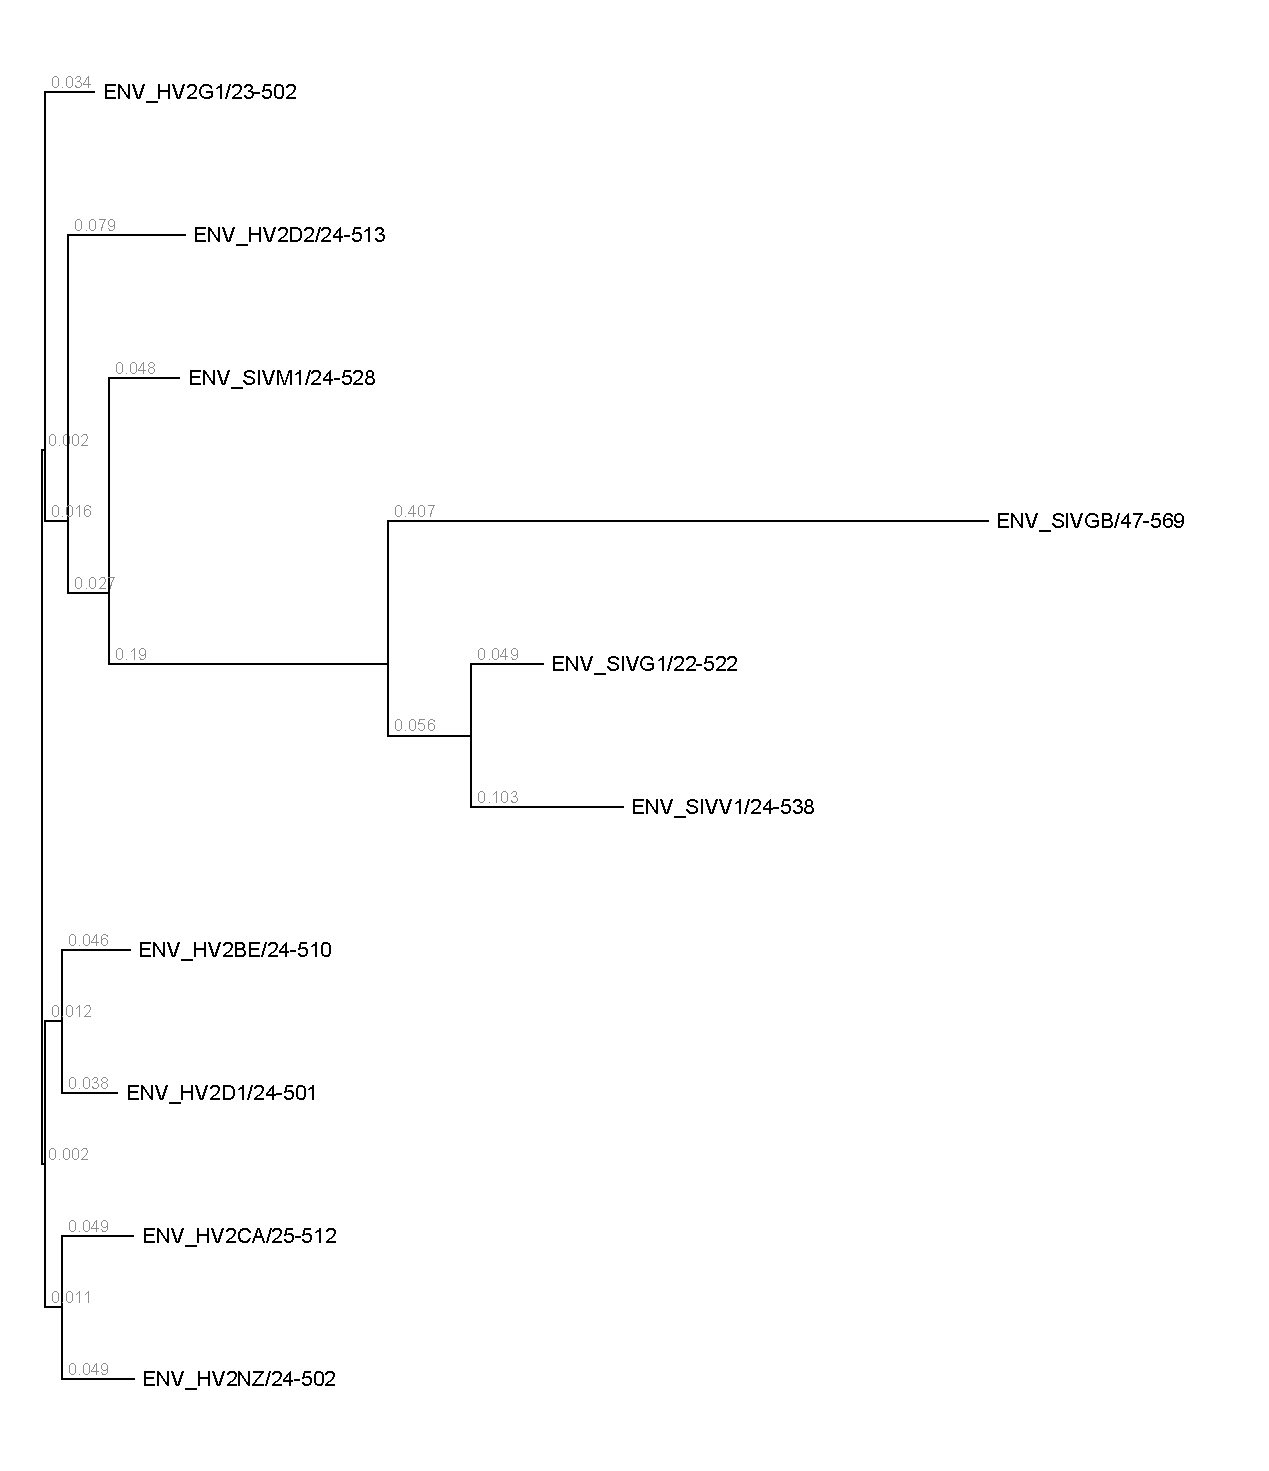
\includegraphics[width=.8\columnwidth]{gp120tree.pdf}
  \caption{
    Tree of selected HIV and SIV GP120 domains, used for the simulation benchmark.
  }
\end{figure}

\begin{figure}
  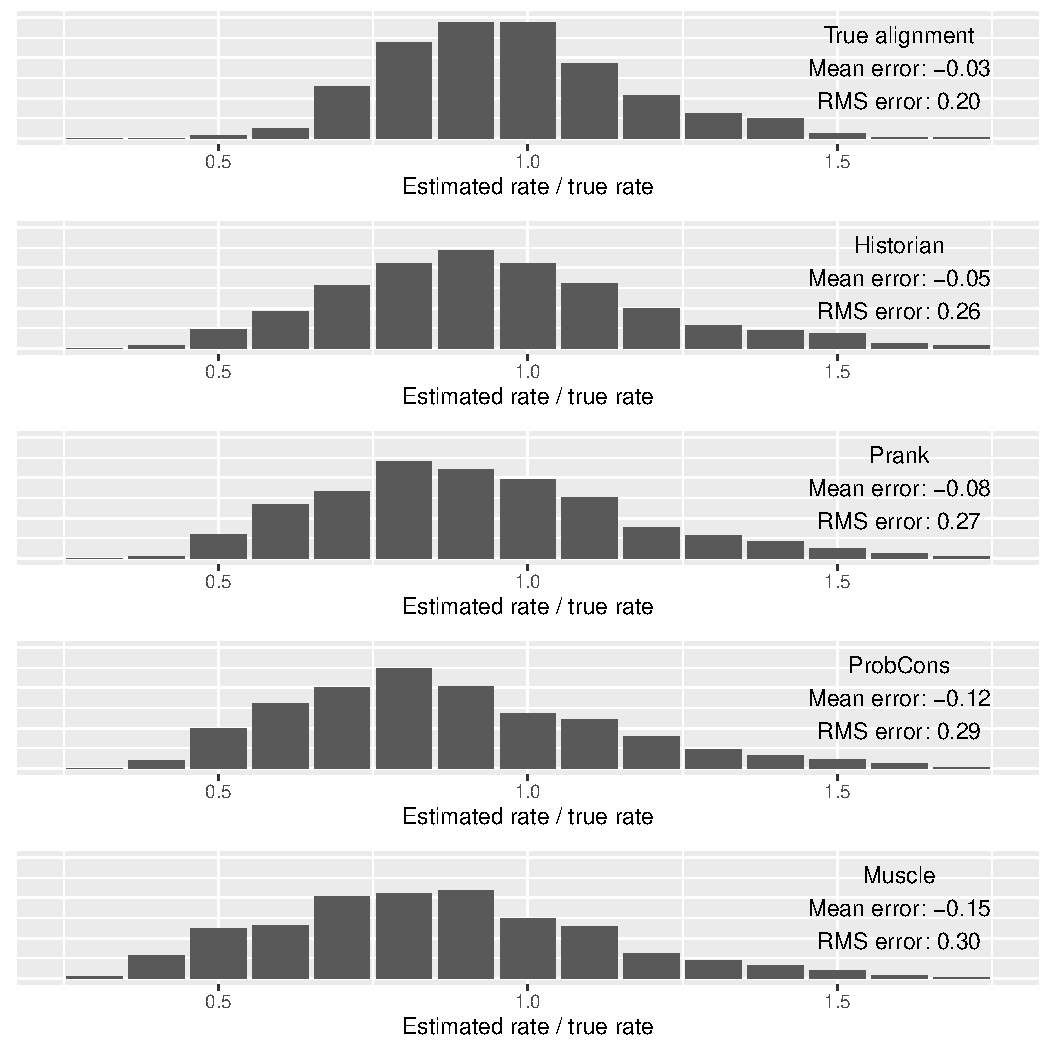
\includegraphics[width=\columnwidth]{sim/results.pdf}
  \caption{
    Results of the simulation benchmark.
    For each method evaluated, the distribution of the ratio of inferred to true
    indel rate is shown; for a perfect rate inference, this ratio would be equal to 1.
    The mean of the ratio is also shown; this represents the the systematic error,
    so e.g. using Muscle results in a systematic 15\% underestimate of indels
    in these simulations.
    The root-mean-squared value of the ratio is also shown,
    and the median and interquartile range are annotated above each plot.
    Tool versions are as shown in Table~1.
  }
\end{figure}

We first performed a simulation benchmark to assess Historian's ability to reconstruct evolutionary parameters,
compared to other tools.
We based the simulation parameters on the evolutionary profile of the HIV/SIV GP120 envelope domain, as follows.
We started with a tree made from an alignment of ten HIV and SIV GP120 domains (Figure~1).
%The resulting tree has three branches that are over 0.1 substitutions/site in length (the relevant branch lengths are 0.10, 0.19, and 0.41).
%The remaining branch lengths were all under 0.1 subs/site; the median branch length was 0.046 subs/site.
We used the tree to estimate the indel rates for the alignment,
and simulated 100 different alignments on this tree
using a sequence length of 500 amino acids
(roughly the same as the GP120 domain)
with the expected substitution rate ($\sigma$) set to one substitution per unit of time
and the simulated insertion and deletion rates ($\lambda,\mu$)
set to the midpoint of the insertion and deletion rates
estimated for GP120 (0.028 indels per unit of time).
For a substitution model, we used the Dayhoff PAM matrix,
which we judged not to give an unfair advantage either to Historian
(which by default uses a matrix estimated from PFAM)
or to Prank (which uses the WAG matrix).

From the simulated sequence data, we estimated indel rates
(a) using the true evolutionary alignment (supplied to Historian);
(b,c) using Historian (alignment-free, default and fast modes);
and
(d,e,f) using Prank, ProbCons and Muscle,
the best-performing tools from the ProtPal benchmark \citep{Westesson2012-zg}.
In each case, we estimated insertion and deletion rates $(\hat{\lambda},\hat{\mu})$ and computed relative errors $(\frac{\hat{\lambda}-\lambda}{\lambda},\frac{\hat{\mu}-\mu}{\mu})$
compared to the simulated indel rates.
Having performed this experiment
using the rates estimated for GP120 ($\sigma=1,\lambda=\mu=0.028$),
we repeated the simulation, varying the rate parameters
($\sigma=2,\lambda=\mu=0.056;
\sigma=5,\lambda=\mu=0.14;
\sigma=2,\lambda=\mu=0.112;
\sigma=5,\lambda=\mu=0.28;
\sigma=5,\lambda=\mu=0.005;
\sigma=5,\lambda=\mu=0.01$)
while still using the tree of Figure~1.
Varying rate parameters did not appear
significantly to affect the ranking of the programs.

The results of this experiment are summarized in Figure~2.
Note that even perfect knowledge of the true evolutionary alignment does not guarantee perfect reconstruction of the underlying indel rate parameters.
Indel events can overlap and thus be under-counted,
leading to a small negative bias in the estimated rate,
and the inherent noisiness of the simulation leads to a spread in the distribution
of estimated rates from individual alignments.
Historian and Prank (which both explicitly aim to provide ancestral reconstructions)
are the most accurate methods for rate estimation,
with a slight edge over ProbCons and Muscle.
Historian's default mode has a slight edge over its fast mode in rate estimation accuracy.

As well as varying the rate parameters,
we also repeated the benchmark on a symmetric 8-taxon binary tree.
This simulation yielded similar patterns:
Historian and Prank are still comparable (with a slight edge to Prank in the
symmetric tree, {\em versus} Historian in the GP120 tree),
followed by ProbCons, followed by Muscle.
As with the tree of Figure~1,
varying simulation parameters did not appear to change the ranking.

\begin{table}
  \begin{tabular}{r|ccc}
    & Mean SPS & Mean TCS & Notes \\
    \hline
    Historian v1.0.2 & 0.822 & 0.497 & \\
    (fast mode) & 0.820 & 0.494 & \\
ClustalW & 0.787 & 0.447 & From {\tt drive5.com} \\
Prank v.100701 & 0.784 & 0.441 \\
%MAFFT & 0.873 & 0.607 \\
ProbCons v1.12 & 0.883 & 0.619 & From {\tt drive5.com} \\
Muscle v3.8.31 & 0.843 & 0.532 & \\
Muscle v4.0 & 0.889 & 0.642 &  From {\tt drive5.com}
  \end{tabular}
  \caption{
    Comparison of Historian to other alignment programs using the BAliBase 3.0 benchmark
    with SPS and TCS alignment quality scores \citep{ThompsonEtAl2005}.
%    Average runtime per alignment was 55s for BAliBase and 39s for PREFAB (4 GHz Intel Core i7).
%    Data for ClustalW, Prank (+F option, ClustalW tree), MAFFT (v6.603), ProbCons (v1.12) and Muscle (version 4.0) are from {\tt http://drive5.com/bench/} \citep{Edgar2010}.
  }
\end{table}

Table~2 summarizes an evaluation of Historian
on the BAliBase 3.0 benchmark,
compiled using 3D structural alignments.
%
In general, Historian performs better on these structure-derived benchmarks than Prank,
which also performs ancestral reconstruction \citep{LoytynojaGoldman2008}.
Compared to leading protein aligners that do not attempt ancestral reconstruction,
Historian outperforms ClustalW \citep{LarkinEtAl2007}, but not Muscle \citep{Edgar2004b}
or ProbCons \citep{DoEtAl2005}. %, or MAFFT \citep{KatohEtAl2005}.
No significant difference was found between Historian's default and fast modes.

\begin{table}
  \begin{tabular}{r|c}
    & Average run time per alignment \\
    \hline
Historian v1.0.2 & 233s \\
 (fast mode) & 55s \\
Prank v.100701 & 520s \\
Muscle v3.8.31 & 1.9s \\
\end{tabular}
\caption{
    Comparison of runtimes of Historian, Prank and Muscle on the BAliBase 3.0 benchmark.
  }
\end{table}

As noted in Table~2, some of the results were taken from the Muscle website, {\tt drive5.com/bench/} \citep{Edgar2010}.
To make a direct comparison of runtimes, we re-ran the benchmarks for Prank and Muscle on the same CPU as the Historian benchmark (Intel Xeon 3.20GHz).
The runtimes are summarized in Table~3: Historian is an order of magnitude slower than Muscle, but an order of magnitude faster than Prank.
Re-running Prank and Muscle resulted in a slight improvement for Prank
and a slight deterioration for Muscle compared to the {\tt drive5.com} data,
presumably due to versioning issues
(the version of Muscle available for download 3.8.31, whereas the data
reported are for version 4.0; conversely, a more recent version of Prank is available
than the one benchmarked on the Muscle website).
Table~2 reflects our results, where available, and the {\tt drive5.com} results in other cases.

We did not benchmark MCMC approaches
such as BaliPhy \citep{Redelings2014}, StatAlign \citep{NovakEtAl2008} or HandAlign \citep{WestessonBarquistHolmes2012}.
These are expected to be more accurate, but generally take much longer.
MCMC samplers may be usefully supplemented by decision-theoretic approaches to summarize a sampling run \citep{HermanEtAl2015}.
Other potential ways to improve accuracy include context-dependent gap penalties, as used by Muscle \citep{Edgar2004b}, % and MAFFT \citep{KatohEtAl2005},
and explicit modeling of tandem duplications \citep{SzalkowskiAnisimova2013}.
Incorporating additional data such as structural annotations may further improve alignments \citep{HermanEtAl2014}.

% The best-performing method Muscle introduces heuristics into its scoring scheme
% that improve accuracy.
% 
% It is harder to incorporate these sorts of modifications into a rigorous phylogenetic model
% primarily because they violate the assumption of independence
% between indel and substitution processes
% that most such models rely on
% 
% Comparison to MCMC tools
% BaliPhy \citep{RedelingsSuchard2005,RedelingsSuchard2007,Redelings2014},
% StatAlign \citep{NovakEtAl2008,HermanEtAl2014},
% HandAlign \citep{WestessonBarquistHolmes2012}
% 
% Decision theory may also be useful to produce consensus alignments summarizing an MCMC run \citep{HermanEtAl2015}



\section{Availability}

Historian is available at \url{github.com/ihh/indelhistorian} under the CC BY 3.0 US license.
Precompiled binaries for Linux or OSX are available.
The program may also be compiled from the C++11 source
on a POSIX system with Clang (v.6.1.0) and several free libaries (libgsl, libz and Boost).
Makefiles to reproduce the analyses reported in this paper
are included in the repository, and the simulation data
are available at \url{github.com/ihh/gp120sim}.

\section*{Acknowledgements}

Historian includes code from Ivan Vashchaev (gason), Heng Li (kseq), % Rafael Baptista (stacktrace), David Robert Nadeau (memsize), Roger Pate (string escaping), Konrad Rudolph (index sort),
and the StackOverflow community.

\section*{Funding}

This work has been supported by NHGRI grant R01-HG004483.

\bibliographystyle{natbib}
%\bibliographystyle{bioinformatics}
%\bibliographystyle{achemnat}
%\bibliographystyle{plainnat}
%\bibliographystyle{abbrv}
%
%\bibliographystyle{plain}
%
%\bibliography{Document}


\bibliography{references}
\end{document}
